\section{Implementation}

In this section, we describe the instantiation of \name on top of off-the-shelf
eventually consistent distributed store Cassandra. We particularly focus on the
challenges in realizing an efficient implementation of our model.

\begin{figure}
\begin{center}
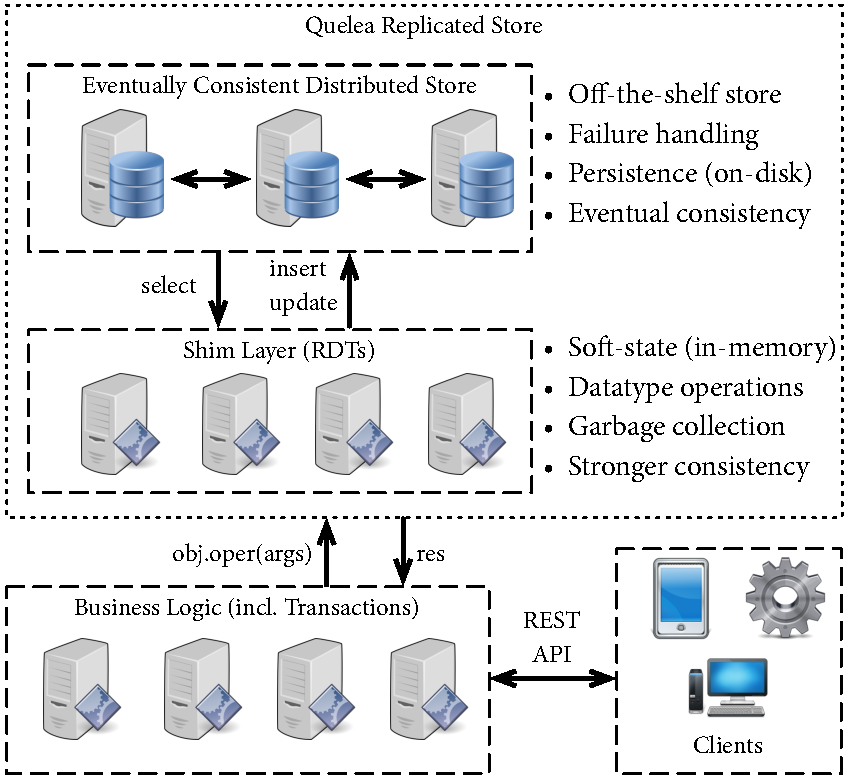
\includegraphics[width=0.9\columnwidth]{Figures/ImplModel}
\end{center}
\caption{Implementation Model.}
\label{fig:impl_mod}
\end{figure}

\name is implemented as a shallow extension of Haskell on the Glasgow Haskell
Compiler (GHC). We utilize Template Haskell functionality to implement static
contract classification. Our proof obligations are discharged automatically
with the help of Z3~\cite{} SMT solver. Figure~\ref{fig:impl_mod} describes the
overall system architecture. The main idea in our implementation of \name is to
offload the majority of concerns related to data management such as
replication, fault tolerance, availability and convergence to Cassandra, an
off-the-shelf eventually consistent store (called \emph{backing store} in the
sequel).

Replicated data type implementation and the stronger consistency semantics are
enforced in the \emph{shim layer}. Our implementation supports eventual, causal
and strong consistency for operations, and RC, MAV and RR transaction
semantics. Complex business logic is implemented with the help of transactions
on the server side, with clients interacting with the web-service over REST
interface. From an engineering perspective, resorting to an off-the-shelf
backing store meant that our entire implementation comprised of only around
2500 lines of Haskell code, which is packaged as a Haskell library\footnote{url
to the hackage}.

% All of this functionality is implemented on top of the standard interface
% exposed by Cassandra, and illustrates the portability of \name programming
% model.
\subsection{Shim Layer}

The shim layer maintains a causally consistent in-memory snapshot of a subset
of objects in the backing store, by explicitly tracking dependencies introduced
between the effects due to visibility, session and same transaction relations.
The dependence tracking is similar to the techniques presented in~\cite{BoltOn}
and~\cite{Eiger}, with the usual optimizations making use of transitivity
properties for minimizing the number of dependencies. Shim layer performs the
reductions associated with replicated datatype operations corresponding to
client requests. As the backing store provides durability, convergence and
fault tolerance, each shim layer node simply acts as a soft-state cache, and
can safely be terminated at any instant. Similarly, more shim layer nodes can
be spawned on demand.

\KC{Perhaps the following two subsections can be elided/shortened?}

\subsection{Operation Consistency}

Every effect generated as a result of an effectful operation on an object
inserts a new row $(o,e,vis,txn,val)$ into the backing store, where $o$ and $e$
are object and (unique) effect identifiers, $vis$ is the set of identifiers of
effects visible to this operation, $txn$ is an optional transaction identifier,
and $val$ is the value associated with the effect (eg: \cf{Withdraw 50}). The
shim layer periodically fetches updates from the backing store for those
objects which were accessed since updates were last fetched. Since causally
consistent operations require an up-to-date view of the current session, the
shim layer node synchronously fetches operations if the causally preceding
operations in the current session are not available in the cache.  Strongly
consistent operations are performed after obtaining exclusive leases on
objects. The lease mechanism is implemented with the help of Cassandra's
support for conditional updates and expiring columns.

\subsection{Transactions}

While Cassandra offers all-or-nothing failure semantics for multiple writes
through batching, readers may witness the initial write while the batch is in
progress. \name implements atomic visibility by exploiting shim layer causality
guarantee -- an effect is included only if all the effects if depends on are
also included.

For every transaction, we instantiate a special transaction marker effect $m$,
but importantly, do not insert into the backing store. $m$ is included as a
dependence to every effect (let $e$ be one such effect) generated in the
transaction. Since $m$ has not yet been written to the store, no operation will
witness $e$ while the transaction in progress. Let $S$ be the set of effects
generated in the transaction. At the end of the transaction, we insert $m$ into
the backing store with $S$ as its dependence. Now any replica which includes
$e$, must include $m$, and transitively must include every effect from the
transaction. This ensures atomicity and satisfies the RC requirement.

The above scheme prevents a transaction from witnessing its own effects. This
might conflict with the causality requirement on the operations. Hence,
transactions piggy-back the previous effects from the same transaction for each
request. MAV semantics is implemented by keeping track of the set of
transaction markers $M$ witnessed by the transaction, and before performing an
operation at some replica, ensuring that $M$ is a subset of the transaction
markers included at that replica. If not, the missing effects are synchronously
fetched. RR semantics is realized by capturing a optimized snapshot of the
state of some replica; each operation from an RR transaction is applied to this
snapshot state. Any generated effects are added to this snapshot.

\subsection{Summarization}

The main challenge in realizing an efficient implementation of operation-based
replicated data types is that the state of the object i.e., the set of effects
grows with every effectful operation on the object. If left unchecked, the
operations slow down over time, until the shim layer memory or backing store
disk runs out of memory. Luckily, the state of the operation-based replicated
data type can often be summarized to an \emph{observably equivalent} smaller
state. For example,

\begin{itemize}
\setlength{\itemsep}{2pt}
\item A last-writer-wins register with multiple updates where $v$ is the value
of the last write is observably equivalent to a register with a single write
$v$.

\item A bank account with a series of deposits and withdraws with current
balance $b$ is equivalent to a bank account with a single deposit of $b$.

\item A set with collection of add and remove operations is equivalent to a set
with a series of add operations of live elements from the original set.
\end{itemize}

Since the semantics of summarization depends on the semantics of the data type,
we expect the programmer to provide a summarization function for each RDT with
the following type:

\begin{codehaskell}
summarize :: Effect e => [e] -> [e]
\end{codehaskell}

\noindent with the intention that the length of the result is smaller that the
length of the argument. We utilize the \cf{summarize} function to summarize the
object state both in the shim layer node and the backing store, typically when
the number of effects on an object crosses a tunable threshold. Shim layer
summarization is straight-forward; a summarization thread takes the local lock
on the object, and replaces its state with the summarized state. The shim layer
node remains unavailable for that particular object during summarization
(usually a few milliseconds).

Compared to the shim layer, summarization in the backing store is more
complicated. The main challenge is that unlike the shim layer, summarization
cannot run as an atomic operation. Summarization in the backing store involves
deleting previously inserted rows and inserting new rows, where each row
corresponds to an effect. It is essential that concurrent client operations are
permitted, but are not allowed to witness the intermediate state of the
summarization process. To this end, we adopt a summarization strategy that
builds on the causality property of the store. The details of the summarization
are beyond the scope of the paper, and is presented in detail in the tech
report~\cite{}.
